\section{Nền tảng Toán học và Xử lý Tín hiệu}
\label{sec:math_and_signal_processing}

\subsection{Giới thiệu: Ngôn ngữ chung để mô tả Thế giới Thị giác}

Thị giác Máy tính, tại cốt lõi của nó, là một nỗ lực nhằm mô tả thế giới vật lý và diễn giải nó thông qua các thuật toán. Để thực hiện được điều này, chúng ta cần một ngôn ngữ chung, chính xác và mạnh mẽ để biểu diễn cả dữ liệu thị giác (ảnh, video) và các phép biến đổi trên chúng. Ngôn ngữ đó chính là Toán học. Các công cụ từ Đại số Tuyến tính, Giải tích, Xác suất Thống kê và Xử lý Tín hiệu không chỉ là những phương tiện kỹ thuật; chúng chính là bộ khung khái niệm cho phép chúng ta định hình vấn đề, thiết kế mô hình, và tối ưu hóa giải pháp.

Trong phần này, chúng ta sẽ đi sâu vào bốn trụ cột toán học và kỹ thuật đã định hình nên lĩnh vực Thị giác Máy tính:
\begin{itemize}
    \item \textbf{Đại số Tuyến tính:} Ngôn ngữ để biểu diễn dữ liệu và các phép biến đổi hình học.
    \item \textbf{Giải tích Đa biến:} Động cơ cho việc tối ưu hóa và học các tham số của mô hình.
    \item \textbf{Xác suất và Thống kê:} Khuôn khổ để mô hình hóa sự không chắc chắn và suy luận từ dữ liệu.
    \item \textbf{Xử lý Tín hiệu:} Cội nguồn của các khái niệm về biểu diễn, lọc và biến đổi tín hiệu hình ảnh.
\end{itemize}
Việc nắm vững những nền tảng này không chỉ giúp bạn hiểu "cách hoạt động" của các thuật toán hiện đại, mà còn trang bị cho bạn tư duy để có thể đọc, hiểu, và tự phát triển các phương pháp mới trong tương lai.

\subsection{Đại số Tuyến tính: Ngôn ngữ của Dữ liệu và Biến đổi}

Nếu có một nhánh toán học nào được coi là "ngôn ngữ mẹ đẻ" của Thị giác Máy tính và Học máy, đó chính là Đại số Tuyến tính. Mọi đối tượng cơ bản trong lĩnh vực này—từ một pixel, một hình ảnh, một video, cho đến một vector đặc trưng hay trọng số của một mạng nơ-ron—đều được biểu diễn và thao tác dưới dạng các cấu trúc đại số tuyến tính.

\subsubsection{Vector: Từ điểm trong không gian đến Vector đặc trưng}
Một vector về cơ bản là một mảng các con số được sắp xếp theo một trật tự. Trong CV, chúng có hai vai trò chính:
\begin{description}
    \item[Biểu diễn điểm hoặc hướng:] Một vector $\mathbf{v} \in \mathbb{R}^n$ có thể được hình dung như một điểm trong không gian $n$-chiều, hoặc một mũi tên bắt đầu từ gốc tọa độ đến điểm đó. Ví dụ, một màu sắc có thể được biểu diễn bằng một vector 3 chiều $\mathbf{c} = [r, g, b]^T$, với mỗi thành phần tương ứng với cường độ của màu đỏ, lục, và lam.
    \item[Biểu diễn đặc trưng (Feature Vector):] Đây là vai trò quan trọng nhất trong học máy. Sau khi một mô hình xử lý một hình ảnh, nó thường tóm tắt toàn bộ thông tin ngữ nghĩa của ảnh đó vào một vector đặc trưng có chiều dài cố định. Ví dụ, một mạng nơ-ron có thể biến đổi một ảnh mèo kích thước $224 \times 224 \times 3$ thành một vector 1024 chiều. Vector này mã hóa các thuộc tính trừu tượng như "có lông", "có tai nhọn", "có bốn chân". Các vector của những ảnh mèo khác nhau sẽ nằm gần nhau trong không gian đặc trưng này.
\end{description}

\textbf{Chuẩn Vector (Vector Norms):} Chuẩn của một vector là một hàm số đo lường "độ lớn" hoặc "chiều dài" của nó. Các chuẩn $L_p$ được định nghĩa là:
\begin{equation}
    \|\mathbf{x}\|_p = \left( \sum_{i=1}^{n} |x_i|^p \right)^{1/p}
\end{equation}
Hai chuẩn phổ biến nhất trong CV là:
\begin{itemize}
    \item \textbf{Chuẩn $L_2$ (Euclidean Norm):} $\|\mathbf{x}\|_2 = \sqrt{\sum x_i^2}$. Đây chính là khoảng cách Euclid thông thường từ gốc tọa độ đến điểm $\mathbf{x}$. Nó thường được sử dụng trong các hàm mất mát, ví dụ như Sai số Toàn phương Trung bình (Mean Squared Error), để đo lường sự khác biệt giữa vector dự đoán và vector thực tế.
    \item \textbf{Chuẩn $L_1$ (Manhattan Norm):} $\|\mathbf{x}\|_1 = \sum |x_i|$. Nó đo lường tổng các giá trị tuyệt đối của các thành phần. Chuẩn $L_1$ có một đặc tính quan trọng là nó thúc đẩy tính thưa (sparsity), tức là làm cho nhiều thành phần của vector tiến về 0. Điều này rất hữu ích trong các kỹ thuật như LASSO regression và Compressed Sensing.
\end{itemize}

\subsubsection{Ma trận: Biểu diễn Ảnh và các Phép biến đổi Tuyến tính}
Một ma trận là một mảng số hai chiều. Trong CV, ma trận có hai vai trò chính:
\begin{description}
    \item[Biểu diễn dữ liệu:] Một ảnh xám (grayscale) có kích thước $H \times W$ có thể được biểu diễn trực tiếp dưới dạng một ma trận $\mathbf{I} \in \mathbb{R}^{H \times W}$, trong đó mỗi phần tử $I_{ij}$ là cường độ sáng của pixel tại hàng $i$ và cột $j$.
    \item[Biểu diễn phép biến đổi tuyến tính:] Một ma trận $\mathbf{A} \in \mathbb{R}^{m \times n}$ có thể được xem như một hàm số biến đổi một vector $\mathbf{x} \in \mathbb{R}^n$ thành một vector mới $\mathbf{y} \in \mathbb{R}^m$ thông qua phép nhân ma trận: $\mathbf{y} = \mathbf{A}\mathbf{x}$. Các phép biến đổi hình học cơ bản như co giãn (scaling), xoay (rotation), trượt (shear) đều có thể được biểu diễn bằng các ma trận biến đổi. Đây là nền tảng của các kỹ thuật tăng cường dữ liệu (data augmentation) và xử lý hình học.
\end{description}

\subsubsection{Tensor: Khái quát hóa cho Dữ liệu Đa chiều}
Trong bối cảnh học sâu hiện đại, khái niệm \textbf{tensor} là cực kỳ quan trọng. Một tensor là sự khái quát hóa của vector và ma trận thành các mảng $n$-chiều. Bậc (rank hay order) của một tensor chính là số chiều của nó.
\begin{itemize}
    \item \textbf{Tensor bậc 0:} Một số vô hướng (scalar).
    \item \textbf{Tensor bậc 1:} Một vector.
    \item \textbf{Tensor bậc 2:} Một ma trận.
    \item \textbf{Tensor bậc 3:} Có thể biểu diễn một ảnh màu. Một ảnh RGB kích thước $H \times W$ được biểu diễn bằng một tensor bậc 3 có kích thước $(H, W, 3)$, trong đó 3 là số kênh màu (Red, Green, Blue).
    \item \textbf{Tensor bậc 4:} Thường dùng để biểu diễn một lô (batch) các ảnh màu. Nếu chúng ta có một lô gồm $N$ ảnh, tensor sẽ có kích thước $(N, H, W, 3)$. Đây chính là định dạng dữ liệu đầu vào tiêu chuẩn cho hầu hết các mạng nơ-ron thị giác.
\end{itemize}
Các thư viện học sâu như PyTorch và TensorFlow đều sử dụng tensor làm cấu trúc dữ liệu cơ bản.

\subsubsection{Phân rã Ma trận: SVD và Phân rã Trị riêng}
Phân rã ma trận là quá trình phân tích một ma trận thành tích của các ma trận thành phần có cấu trúc đặc biệt.
\begin{description}
    \item[Phân rã Trị riêng (Eigendecomposition):] Cho một ma trận vuông $\mathbf{A}$, phân rã trị riêng tìm ra các vector riêng (eigenvectors) $\mathbf{v}$ và trị riêng (eigenvalues) $\lambda$ thỏa mãn $\mathbf{A}\mathbf{v} = \lambda\mathbf{v}$. Trực giác, vector riêng là những hướng mà phép biến đổi $\mathbf{A}$ chỉ co giãn mà không làm thay đổi hướng. Phân rã trị riêng là nền tảng của thuật toán Phân tích Thành phần Chính (Principal Component Analysis - PCA), một kỹ thuật giảm chiều dữ liệu kinh điển.
    \item[Phân rã Giá trị suy biến (Singular Value Decomposition - SVD):] SVD là một kỹ thuật phân rã mạnh mẽ hơn, áp dụng được cho mọi ma trận (không cần vuông). Nó phân rã ma trận $\mathbf{A}$ thành $\mathbf{A} = \mathbf{U}\mathbf{\Sigma}\mathbf{V}^T$. SVD cho phép chúng ta tìm ra các "hướng" quan trọng nhất trong dữ liệu và được sử dụng rộng rãi trong các bài toán như nén ảnh, khử nhiễu, và đề xuất hệ thống.
\end{description}

\subsection{Giải tích Đa biến: Động cơ của Tối ưu hóa và Học tập}

Nếu Đại số Tuyến tính cung cấp các cấu trúc dữ liệu, thì Giải tích Đa biến cung cấp các công cụ để "học" từ dữ liệu đó. Quá trình huấn luyện một mô hình học sâu về bản chất là một bài toán tối ưu hóa khổng lồ: tìm ra bộ tham số (trọng số) của mô hình sao cho hàm mất mát (loss function) đạt giá trị nhỏ nhất.

\subsubsection{Gradient: Hướng đi của sự Tối ưu}
Trong giải tích một biến, đạo hàm $f'(x)$ cho ta biết độ dốc của hàm số tại một điểm. Trong không gian nhiều chiều, khái niệm tương đương là \textbf{gradient}.
Gradient của một hàm số nhiều biến $L(W)$, ký hiệu là $\nabla_W L$, là một vector chứa tất cả các đạo hàm riêng của $L$ theo từng thành phần của $W$.
\begin{equation}
    \nabla_W L = \left[ \frac{\partial L}{\partial w_1}, \frac{\partial L}{\partial w_2}, \dots, \frac{\partial L}{\partial w_n} \right]^T
\end{equation}
\textbf{Trực giác quan trọng nhất:} Vector gradient $\nabla_W L$ tại một điểm luôn chỉ về hướng mà hàm số $L$ \textbf{tăng nhanh nhất}. Do đó, vector \textbf{âm gradient} $(-\nabla_W L)$ sẽ chỉ về hướng mà hàm số $L$ \textbf{giảm nhanh nhất}.

\subsubsection{Hạ Gradient (Gradient Descent)}
Đây là thuật toán tối ưu hóa nền tảng nhất và phổ biến nhất trong học sâu. Ý tưởng của nó vô cùng đơn giản và trực quan, giống như việc một người đi xuống một thung lũng trong sương mù: tại mỗi bước, bạn tìm hướng dốc nhất xuống dưới và đi một bước nhỏ theo hướng đó.
\begin{center}
    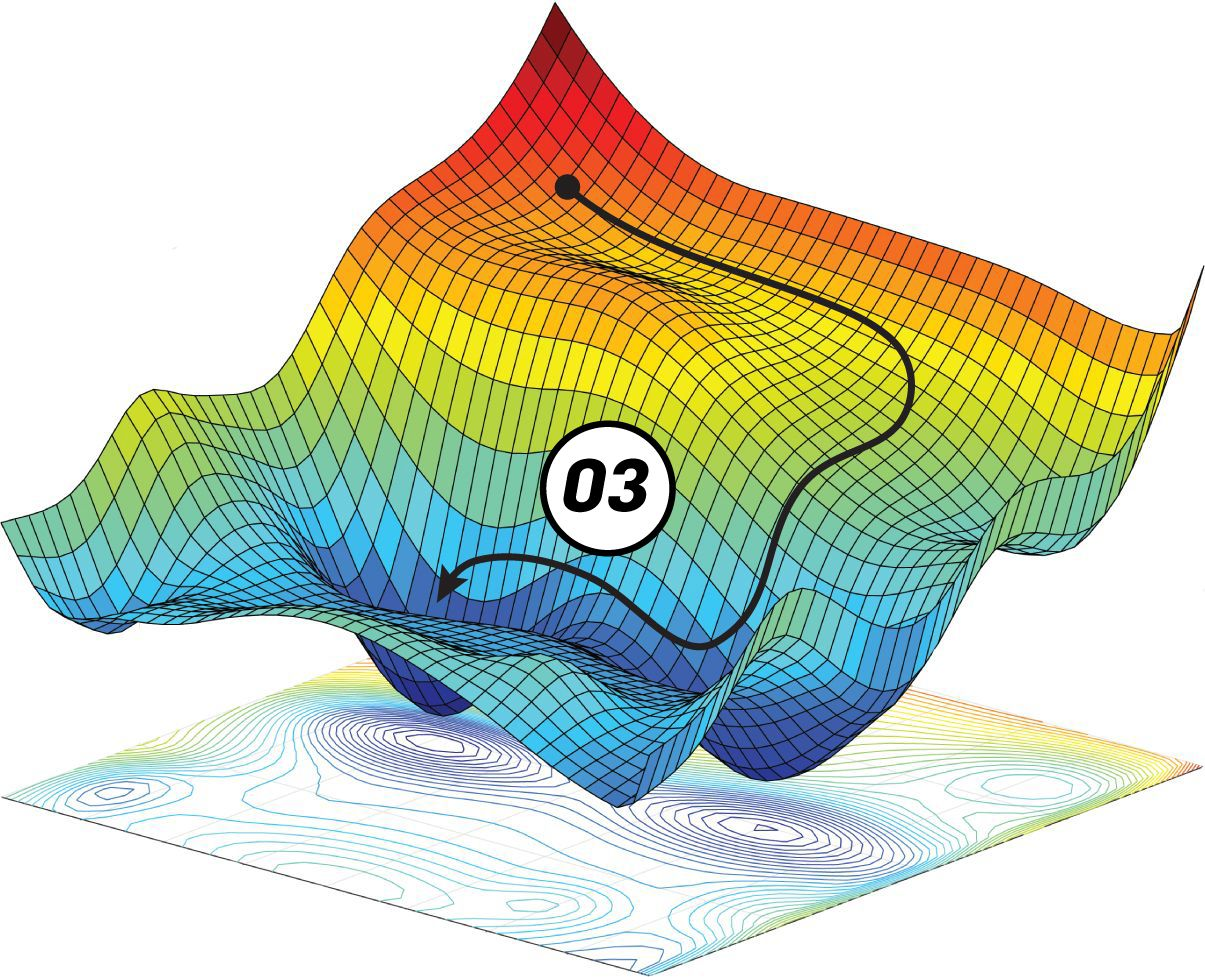
\includegraphics[width=0.7\textwidth]{images/gradient_descent.jpg}
    \captionof{figure}{Minh họa thuật toán Hạ Gradient. Bắt đầu từ một điểm ngẫu nhiên trên bề mặt của hàm mất mát, thuật toán lặp đi lặp lại việc di chuyển một bước nhỏ theo hướng ngược lại với gradient (hướng dốc nhất) để tiến dần đến điểm cực tiểu.}
    \label{fig:gradient_descent}
\end{center}
Quy trình huấn luyện một mô hình sử dụng Hạ Gradient:
\begin{enumerate}
    \item Khởi tạo các trọng số $W$ của mô hình một cách ngẫu nhiên.
    \item Lặp lại cho đến khi hội tụ:
    \begin{enumerate}
        \item Tính toán giá trị của hàm mất mát $L(W)$ trên tập dữ liệu huấn luyện.
        \item Tính toán vector gradient của hàm mất mát theo các trọng số: $\nabla_W L$.
        \item Cập nhật các trọng số bằng cách đi một bước nhỏ theo hướng âm gradient:
        \begin{equation}
            W_{\text{new}} = W_{\text{old}} - \eta \nabla_W L
            \label{eq:gradient_descent}
        \end{equation}
        Trong đó $\eta$ là \textbf{tốc độ học (learning rate)}, một siêu tham số (hyperparameter) quan trọng quyết định độ lớn của mỗi bước cập nhật.
    \end{enumerate}
\end{enumerate}

\subsubsection{Quy tắc Chuỗi và Lan truyền Ngược (Chain Rule \& Backpropagation)}
Một mạng nơ-ron sâu có thể được xem như một hàm hợp cực kỳ phức tạp: $L(f_k(\dots f_2(f_1(\mathbf{x}, W_1), W_2)\dots), W_k))$. Làm thế nào để tính được gradient của hàm mất mát cuối cùng $L$ theo các trọng số $W_1$ ở lớp đầu tiên?
Câu trả lời nằm ở \textbf{quy tắc chuỗi (chain rule)} trong giải tích. Nó cho phép chúng ta tính đạo hàm của một hàm hợp bằng cách nhân các đạo hàm của các hàm thành phần.
\textbf{Lan truyền ngược (Backpropagation)} là một thuật toán thông minh và hiệu quả để áp dụng quy tắc chuỗi trên toàn bộ mạng nơ-ron. Nó tính toán gradient từ lớp cuối cùng ngược trở về các lớp đầu tiên, giống như một dòng chảy thông tin ngược, cho phép tính toán hiệu quả $\nabla_W L$ cho tất cả các trọng số trong mạng. Đây chính là thuật toán cốt lõi cho phép chúng ta huấn luyện các mạng nơ-ron sâu với hàng tỷ tham số.

\subsection{Xác suất và Thống kê: Khuôn khổ cho Sự không chắc chắn}

Thế giới thực vốn không chắc chắn và dữ liệu thị giác luôn chứa nhiễu. Xác suất và Thống kê cung cấp một bộ công cụ để mô hình hóa sự không chắc chắn này, suy luận từ dữ liệu, và đưa ra các dự đoán mang tính xác suất.

\begin{description}
    \item[Phân loại như một bài toán suy luận xác suất:] Thay vì đưa ra một dự đoán chắc chắn "đây là con mèo", một mô hình phân loại hiện đại thường đưa ra một phân phối xác suất trên các lớp: $P(\text{class}|\text{image})$, ví dụ: (mèo: 95\%, chó: 4\%, hổ: 1\%).
    \item[Mô hình hóa dữ liệu:] Các mô hình sinh (generative models) như GANs hay Diffusion Models học cách mô hình hóa phân phối xác suất của chính dữ liệu, $P(\text{image})$. Điều này cho phép chúng tạo ra các mẫu dữ liệu mới (ảnh mới) trông giống như dữ liệu huấn luyện.
    \item[Định lý Bayes:] Là nền tảng cho suy luận thống kê. Nó cho phép chúng ta cập nhật niềm tin (xác suất) của mình về một giả thuyết khi có bằng chứng mới.
    \begin{equation}
        P(H|E) = \frac{P(E|H)P(H)}{P(E)}
    \end{equation}
    Trong đó, $P(H|E)$ (xác suất hậu nghiệm) là xác suất của giả thuyết $H$ sau khi quan sát bằng chứng $E$.
    \item[Ước lượng Hợp lý Cực đại (Maximum Likelihood Estimation - MLE):] Là một nguyên lý nền tảng để huấn luyện các mô hình thống kê. Ý tưởng là: chọn các tham số của mô hình sao cho xác suất sinh ra (likelihood) dữ liệu huấn luyện đã quan sát được là lớn nhất. Nhiều hàm mất mát phổ biến (như Cross-Entropy) có thể được diễn giải dưới góc độ của MLE.
\end{description}

\subsection{Xử lý Tín hiệu: Cội nguồn của Biểu diễn và Phép toán}

Trước khi học sâu thống trị, Thị giác Máy tính được xem là một nhánh của Xử lý Tín hiệu. Hình ảnh được coi là các tín hiệu hai chiều, và các công cụ từ lĩnh vực này vẫn còn nguyên giá trị và là nền tảng cho nhiều khái niệm hiện đại.

\subsubsection{Lấy mẫu và Lượng tử hóa}
Một hình ảnh kỹ thuật số là một phiên bản rời rạc của thế giới tương tự (analog). Quá trình này bao gồm hai bước:
\begin{itemize}
    \item \textbf{Lấy mẫu (Sampling):} Rời rạc hóa không gian. Tín hiệu liên tục trong không gian được lấy mẫu tại các vị trí trên một lưới, tạo ra các pixel. Định lý lấy mẫu Nyquist-Shannon cho biết tần số lấy mẫu tối thiểu cần thiết để có thể tái tạo lại tín hiệu gốc một cách hoàn hảo.
    \item \textbf{Lượng tử hóa (Quantization):} Rời rạc hóa giá trị. Cường độ sáng hoặc màu sắc liên tục tại mỗi pixel được làm tròn thành một trong một tập hợp các giá trị hữu hạn (ví dụ: 256 mức từ 0 đến 255 cho ảnh 8-bit).
\end{itemize}

\subsubsection{Phép Tích chập (Convolution)}
Đây là khái niệm quan trọng nhất từ xử lý tín hiệu được kế thừa và phát triển trong học sâu. Phép tích chập là một phép toán tuyến tính, trong đó một "bộ lọc" hay "nhân" (kernel) nhỏ được trượt qua toàn bộ tín hiệu đầu vào, và tại mỗi vị trí, tích chập được tính bằng tổng của tích các phần tử tương ứng.

Trong xử lý tín hiệu 1D rời rạc, nó được định nghĩa là:
\begin{equation}
    (f * g)[n] = \sum_{m=-\infty}^{\infty} f[m]g[n-m]
\end{equation}
Trong xử lý ảnh 2D, nó trở thành:
\begin{equation}
    (I * K)[i, j] = \sum_{m}\sum_{n} I[m, n]K[i-m, j-n]
\end{equation}
\textbf{Trực giác:} Phép tích chập cho phép một kernel nhỏ thực hiện một tác vụ cục bộ (như phát hiện cạnh, làm mờ, làm sắc nét) trên toàn bộ hình ảnh. Chính ý tưởng này đã được Mạng Nơ-ron Tích chập (CNN) kế thừa, trong đó các kernel không còn được thiết kế thủ công mà được "học" trong quá trình huấn luyện.

\subsubsection{Miền Tần số và Biến đổi Fourier}
Biến đổi Fourier là một công cụ toán học cực kỳ mạnh mẽ cho phép chúng ta phân tích một tín hiệu thành các thành phần tần số cấu thành nó. Trực giác, nó chuyển đổi biểu diễn của tín hiệu từ miền không gian ("tín hiệu thay đổi như thế nào theo vị trí") sang miền tần số ("tín hiệu chứa những tần số nào").
\begin{itemize}
    \item Nó cho phép thực hiện các phép lọc tần số, ví dụ như loại bỏ các tần số cao (nhiễu) hoặc giữ lại các tần số thấp (cấu trúc chính).
    \item Một tính chất quan trọng là phép tích chập trong miền không gian tương đương với phép nhân từng phần tử trong miền tần số, giúp tăng tốc độ tính toán cho các kernel lớn.
    \item Các định dạng nén ảnh như JPEG sử dụng các biến thể của biến đổi Fourier (như Biến đổi Cosine Rời rạc - DCT) để loại bỏ các thông tin tần số cao mà mắt người ít nhạy cảm.
\end{itemize}

\section*{Tài liệu tham khảo}
\begin{itemize}
    \item[1] Strang, G. \textit{Introduction to Linear Algebra}. 5th ed. Wellesley-Cambridge Press, 2016.
    \item[2] Goodfellow, I.; Bengio, Y.; Courville, A. \textit{Deep Learning}. MIT Press, 2016. (Đặc biệt là Phần I: Nền tảng Toán học và Học máy)
    \item[3] Szeliski, R. \textit{Computer Vision: Algorithms and Applications}. 2nd ed. Springer, 2022. (Phụ lục A cung cấp một bản tóm tắt toán học tuyệt vời)
    \item[4] Oppenheim, A. V.; Schafer, R. W. \textit{Discrete-Time Signal Processing}. 3rd ed. Pearson, 2009.
    \item[5] Bishop, C. M. \textit{Pattern Recognition and Machine Learning}. Springer, 2006.
    \item[6] Abo-Zahhad, M. M.; Hussein, A. I.; Mohamed, A. M. Compressive Sensing Algorithms for Signal Processing Applications: A Survey. \textit{International Journal of Communications Network and System Sciences} \textbf{2015}, \textit{8}, 197-216.
    \item[7] Lee, H. \textit{Introduction to Compressed Sensing With Coding Theoretic Perspective}. GIST, 2011.
    \item[8] Liu, J.; Jin, Y. A comprehensive survey of robust deep learning in computer vision. \textit{Journal of Automation and Intelligence} \textbf{2023}, \textit{2}, 175-197.
\end{itemize}